% !TEX root = ../thesis.tex
So far we have explained some neural network building blocks and some techniques for reduced complexity. We have run some experiments to better understand some of these techniques. In this chapter, we are going to talk about these experiments and tools we had to built to run these experiments. First we identified some methods and to understand them better, we ran experiments on them. Then we have combined these methods to come up with a model. 

\section{Pruning}
Since pruning individual weights do not effect complexity directly, we are going to focus on pruning nodes from layers. To do that, as \cite{Hu:2016aa} explained, we are going to use \textit{training cycles}. First, we will define a neural network and some data. Then we will train this network using the training dataset. After the training is done, we will run inference for the training dataset and collect ReLU output statistics. Using these statistics, we will try to understand which nodes have minimal effect on accuracy. We will prune these nodes by removing the relevant dimensions from weight matrices. Then we will go back to the training step. We will keep iterating over this list until there are no nodes to be pruned.

\subsection{Fully Connected Summation}
For the sake of simplicity, we started with a very easy problem. We have implemented a neural network consisting of 2 input dimensions ($x_n \in \mathbb{R}^{2}$), one fully connected layer with 1000 nodes and a one fully connected output with a single node ($y_n \in \mathbb{R}$). We have defined the output as the summation of two inputs, ($y_n = x_{n,1} + x_{n,2}$). So that we precisely know the optimum neural network structure that would be able to perform this calculation. Which is a neural network with one fully connected layer with one node and an output layer fully connected to that. All weights equal to $1$ and all biases equal to $0$.

We have calculated the loss using mean squared error, and used Momentum Optimizer (learning rate $0.01$ and momentum $0.9$) to learn the weights. We have generated $1.000.000$ samples, we trained the network with batch size $1000$.

\subsection{MNIST Autoencoder}
To expand our pruning experiments to convolutional neural networks, we have implemented an autoencoder for MNIST Dataset. An autoencoder consists of two parts. First is the encoder, which aims to reduce the dimensionality of input. The other is decoder, which aims to convert the encoded data back to it's original form. Therefore an autoencoder reduces the dimensions of an input data and then tries to recreate that data from those reduced dimensions.

We have defined the auto encoder with two encoder layers followed by two decoder layers. Each encoding layer running a convolution with kernel size $3$ and stride of $2$. Following each of these, we are applying batch normalization and ReLU activation. Each decoding layer is running deconvolutions with kernel size $3$ and stride of $2$. Followed by adding bias, batch normalization and ReLU activations.   
\todoin{confirm the configuration above}

The information contained in one input image $x_n \in \mathbb{R}^{28 \times 28 \times 1}$ is represented with $784$ floating points. Therefore, a good auto-encoder should be reducing this number with each encoding layer. Similarly, converting encoded image back to it's original form with minimal loss while decoding. 

Since we will try to find and prune unused nodes, we will start with a configuration that is larger than necessary. 
\begin{equation*}
\begin{split}
x_n &\in \mathbb{R}^{28 \times 28 \times 1}\\
\psi_1^{(Conv)}:& \mathbb{R}^{28 \times 28 \times 1} \rightarrow \mathbb{R}^{14 \times 14 \times 32} \\
\psi_2^{(Conv)}:& \mathbb{R}^{14 \times 14 \times 32} \rightarrow \mathbb{R}^{7 \times 7 \times 64} \\
\psi_3^{(Deconv)}:& \mathbb{R}^{7 \times 7 \times 64} \rightarrow \mathbb{R}^{14 \times 14 \times 32} \\
\psi_4^{(Deconv)}:& \mathbb{R}^{14 \times 14 \times 32} \rightarrow \mathbb{R}^{28 \times 28 \times 1} \\
L =& RMSE(x_n, \hat y_n)
\end{split}
\end{equation*}

\subsection{Regularization}
In both experiments, we test no regularization, L1 regularization and L2 regularization to see if they effect the activation statistics and pruning.

\subsection{Distortion}
In case of two nodes in one layer, if the weights connecting to them are proportional, it may not be possible to prune one of them. To prevent that, we introduce a little bit distortion, forcing the differentiation of features represented by nodes. 

\subsection{Activations}
We test 3 pruning configurations for activation counts, activation values and activation correlations. 
\todoin{we need proper mathematical notations to be able to describe these properly. We need to be able to define all training samples as a set and as individuals.}

\subsubsection{Activation Counts}
We count the ReLU activations per node. Using this information we determine which nodes are necessary.

\subsubsection{Activation Values}
We collect statistics about activation values per node. Using this information we determine which nodes are necessary.

\subsubsection{Activation Correlation}
We collect statistics about activation correlations to see which nodes are activated together most of the times. Using this information we determine which nodes represent similar features. 


\section{Convolution Operation Alternatives}
In general, convolution operations are expensive. In this section, we experiment with \textit{kernel composition} and \textit{separable convolutions} to see which one is the better alternative to regular convolutions. To see the differences between both operations, we ran two experiments for each. One classifying MNIST dataset, the other classifying CIFAR10 dataset.

We have defined a network with three convolutional layers followed by one fully connected layer. Each convolutional layer has kernel size 5. Convolutional layers are followed by batch normalization, then ReLU activations. First two convolution layers are followed by an average pooling layer with kernel size $2$ and strides of $2$. The third convolutional layer is followed by a global average pooling layer, where we reduce the width and height dimensions to the average of all values in those dimensions. We using SCE loss and momentum optimizer (learning rate $10^{-4}$, and momentum $0.9$), we train this network for $20000$ steps with batch size $32$. 

\begin{equation*}
\begin{split}
x_n &\in \mathbb{R}^{32 \times 32 \times 1}\\
\psi_1^{(Conv)}:& \mathbb{R}^{32 \times 32 \times 3} \rightarrow \mathbb{R}^{32 \times 32 \times 32} \\
\psi_2^{(Conv)}:& \mathbb{R}^{16 \times 16 \times 32} \rightarrow \mathbb{R}^{16 \times 16 \times 64} \\
\psi_3^{(Conv)}:& \mathbb{R}^{8 \times 8 \times 64} \rightarrow \mathbb{R}^{8 \times 8 \times 128} \\
\psi_4^{(FC)}:& \mathbb{R}^{1 \times 1 \times 128} \rightarrow \mathbb{R}^{10} \\
L =& SCE(x_n, \hat y_n)
\end{split}
\end{equation*}
\todoin{this is missing the pooling layers and global average pooling}

By changing $\psi_{(k)}^{(Conv)}$ with $\psi_{(k)}^{(ConvCompose)}$ and $\psi_{(k)}^{(Separable)}$ we obtain 3 versions of this model. Please remember that $\psi_{(k)}^{(ConvCompose)}$ requires an additional parameter for number of intermediate output channels. We use the number of output channels for that. We train each configuration for both MNIST and CIFAR-10 for a fair comparison.

\begin{figure}
\vspace{-65px}
  \begin{center}
        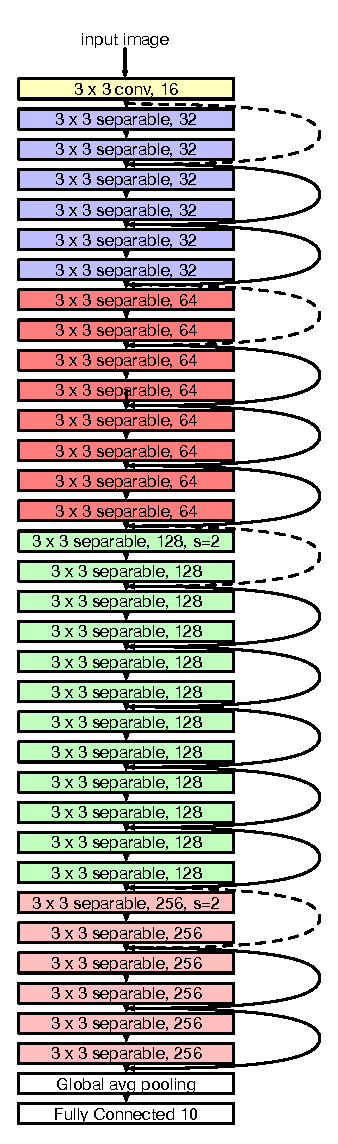
\includegraphics{images/separable_resnet.eps}
  \end{center}
  \caption{Separable Resnet-34. Branching lines represent residual connections, dashed ones are padded with zeros to match the number of channels. If s=2, depthwise convolution is ran with strides of two and residual branch is average pooled with strides 2 and kernel size 2. ReLU and Batch Normalization operations are hidden.}
  \label{fig:model}
\end{figure}
\section{Separable Resnet}
Inspired by ResNet (\cite{He:2015aa}, ), we have created a convolutional neural network with residual connections. In Figure \ref{fig:model} we show the architecture of our neural network. 

\subsection{Design Choices}
\begin{figure}
\vspace{-65px}
\begin{center}
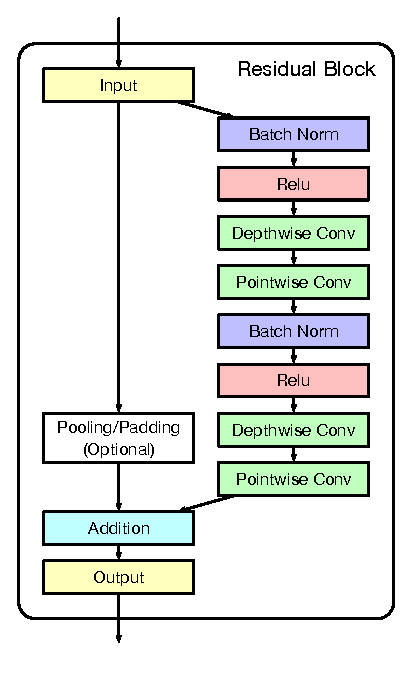
\includegraphics[width=0.38\textwidth]{images/full_preactivation.eps}
\end{center}
\caption{Full pre-activation residual connections.}
\label{fig:full-preactivation}
\end{figure}

\begin{itemize}
\item Except for the first convolutional operation, we have replaced every convolution layer with a separable convolution layer. The first layer has 3 input and 16 output channels. Therefore, for this layer the number of FLOP for a convolution operation ($K*K*m_{k-1}*m_k = 3*3*3*16 = 432$) is not sufficiently higher than a separable convolution ($K*K*m_{k-1} + m_{k-1}m_k = 3*3*3 + 3*16=75$). But for this layer, separable convolution comes with a disadvantage. By definition, it applies a depthwise convolution for color channels separately. We believe that the feature representations of the input are highly dependent on the color channels, therefore we argue that applying a depthwise convolution without mixing the colors is inefficient.
\item ResNet-34 starts with a $7 \times 7$ convolutional kernel with strides of $2$. It is followed by a pooling layer with strides of 2. In our model we chose not to reduce the image size that early. We think that these two layers with strides of $2$ are used to speed up the network and kernel size 7 is used to minimize the loss of information. We argue that this early application of strides will lead to loss of information. 
\item As \cite{he2016identity} proposed, we are using full pre-activation residual connections. See Figure \ref{fig:full-preactivation}.
\end{itemize}

\subsection{Training}
We train our network using CIFAR-10 dataset. We divided the dataset for 50.000 training images and 10.000 validation images. We use momentum optimizer with momentum $0.9$ and learning rates $0.1$, $0.01$, $0.001$ for steps $0$ to $40.000$, $40.000$ to $60.000$ and $60.000$ to $80.000$ respectively. We have defined the loss as SCE of the truth and prediction with an addition of L2 norm of weights multiplied by $0.0002$. We trained our model using the training images for $80.000$ steps with batch size $128$. 

\subsection{Pruning Nodes}
\subsubsection{Pruning Residual Connections}
The addition operation in the residual block creates a one-to-one relationship between different blocks. With the existence of such a relationship, it is not possible to prune a residual block's output nodes. Therefore we first group the residual blocks that are directly connected to each other. We consider the residual blocks that don't apply pooling/padding operation to be directly connected to the previous residual block. Then we calculate the indexes of nodes to keep in the output of every residual block. We union these indexes and prune the remaining nodes from the outputs of every directly connected residual block. We also prune the outputs of first pointwise convolution in the residual blocks separately. 

\subsubsection{Pruning with Adam Optimizer}
We have trained our network using Adam Optimizer (\cite{kingma2014adam}) as well. Adam optimizer keeps two moment matrices for each weight matrix. Therefore, if we are pruning the weights, we prune these matrices.

\subsection{Pruning Weights}
We set weight values that are very close to $0$ to $0$. By doing so, we see the difference in accuracy. Despite the fact that this operation does not change computational complexity, when combined with other methods (i.e. factorization), it will be useful. 

\subsection{Factorization}
We factorize the trained and pruned model. Using SVD we try to decompose the convolution, pointwise convolution and fully connected weights. To do that, we calculate $U$, $S$ and $V$ for each of the weight matrices. From $S$ we pick the most important values that are bigger than threshold value ($\epsilon$). If the decomposed weight matrix would reduce the number of operations, we replace the layer with two new layers, applying the decomposed weights consecutively. We experiment with two versions of this threshold value. One for determining values that are sufficiently small ($\epsilon = 10^{-3}$) and other for finding outliers ($\epsilon = \text{E}[S] - \text{Var}(S)$).

\subsection{Quantization}
We quantize the weights from 32-bits to 8-bit and run performance and accuracy benchmarks.



